\documentclass[conference]{IEEEtran}
%\IEEEoverridecommandlockouts
% The preceding line is only needed to identify funding in the first footnote. If that is unneeded, please comment it out.
\usepackage{cite}
\usepackage{amsmath,amssymb,amsfonts}
\usepackage{algorithm}
\usepackage{algorithmic}
\usepackage{graphicx}
\usepackage{textcomp}
\usepackage{listings}
\usepackage{fancyvrb}
\usepackage{xcolor}
\usepackage[makeroom]{cancel}
\def\BibTeX{{\rm B\kern-.05em{\sc i\kern-.025em b}\kern-.08em
    T\kern-.1667em\lower.7ex\hbox{E}\kern-.125emX}}
\begin{document}

\title{Adapting VBASBS Queueing Model for Proof-of-Stake Consensus Algorithm}

\author{
  \textbf{Kyle Kentner, Nathan Crosby, Andrew Smith, Sush Chittibabu, and Abdulla Karjikar}\\
  Oklahoma State University - Stillwater, OK \\
  kyle.kentner@okstate.edu, ncrosby@okstate.edu, scu@okstate.edu, \\
  sushmitha.chittibabu@okstate.edu, abdulla.karjikar@okstate.edu}

\maketitle

\begin{abstract}

Our main goal with this work is to establish a theoretical model that can simulate
more accurately how blockchain transactions are grouped, validated, processed,
and purged from a network based on a proof-of-stake consensus algorithm. With 
the switch from proof-of-work consensus algorithm to the newer proof-of-stake with 
cryptocurrencies, most notably Ethereum, there is a need to update the theoretical 
models that are used to define efficiency metrics. Further we took it upon ourselves 
to move beyond that and quantify the optimal time window to decrease waiting time
for the average owner of each transaction, while not significantly deteriorating throughput
for the network as a whole.

\end{abstract}

\begin{IEEEkeywords}
Blockchain, Optimization, Queueing
\end{IEEEkeywords}

\section{Introduction}\label{Intro}

The blockchain, a distributed ledger utilizing records linked together via cryptographic 
hashes, has within the last decade captivated the industry. Having been utilized in the 
development of a decentralized economic transfer scheme with the adoption of 
Bitcoin\cite{2008_Bitcoin_Nakamoto}, the original proof-of-work concept had established 
a means of validating incoming transactions through a distributed network of participants. 
This led to the development of other crypto-currency applications, most notably Ethereum. 
These solutions implemented methods with a focus on accuracy and redundancy of the 
various transactions with minimal effort given to reduce individual transactional waiting 
time and increase efficiency of processing transactions.

This approach remains true for Bitcoin; however, Ethereum changed this consensus 
mechanism in 2022 with the update to proof-of-stake\cite{2022_Ethereum_PoS}. This 
changed the blockchain to be more efficient in reducing complexity in the work 
computations while decreasing the barrier to entry hence providing reduced centralized 
risk with the potential of more nodes securing the network. Where under the proof-of-work
consensus algorithm, the timing of blocks was determined by the mining difficulty, the 
new approach, proof-of-stake, the timing is fixed. Time in the Ethereum proof-of-stake 
consensus algorithm is divided into slots of 12 seconds and epochs of 32 slots.

While the proof-of-stake greatly improved the efficiency of transactions, there remains 
room for improvements in the validation of transactions. In this paper, we propose an 
algorithm to decrease waiting time while maintaining a high level of throughput. To begin 
the optimization process, we must first choose a performance model that analytically 
describes the relationship between the number of transactions, the fixed time for those 
transactions to be processed, and the total number of transactions that are processed 
(throughput). Once a representative performance model has been chosen, an optimal
time window can be selected that balances out the throughput. 

Our paper is organized as follows. In section two we conduct a brief literature review and 
then focus on the performance model that will underly our own work. Section three is 
dedicated to the methodology we used to optimize the block size with details of our 
approach theorized via mathematical models. Section four, we discuss the results recorded 
from our early attempts at simulating our proposed model. Then we conclude in section five 
with remarks and discuss potential future areas to continue expanding upon the model. 

\section{Related Work}\label{related}

One of the main detriments of the concept of cryptocurrencies has been the slow transaction
rates with proof-of-work consensus algorithm validation of transactions. The main focus to rectify 
this problem while maintaining the original consensus algorithm can be seen in previous work such 
as Fu\cite{2020_IEEEToVT_Fu}. This work states that when considering blockchain optimization, 
the throughput, or number of transactions processed by a blockchain system in a given amount of 
time, are key indicators of its performance. Mechkaroska\cite{2018_TELFOR_Mechkaroska} explores
some of the methods tried up to that point. They include increasing the block size to increase the 
number of transactions being processed, which is increasing throughput, and a technique called 
"sharding" that is similar to parallel processing of transactions. This showed up in an alt-coin named 
Zilliqa\cite{2017_Zilliqa_Zilliqa} which is mentioned in the paper. While sharding is on the docket of 
potential changes to the Ethereum network, it has not been given the green light yet, and might not
be necessary considering the changes made to the consensus algorithm, discussed later.

The prevalence of articles that called for an increase to the block size to a na\"ive larger size shows 
a lack of creativity to solve this issue of slow transaction validation as can be seen in Gobel, Thakkar, 
and Mechkaroska\cite{2017_IEEE_Gobel, 2018_IEEE_Thakkar, 2018_TELFOR_Mechkaroska}. The 
hard fork in Bitcoin to create Bitcoin Cash was chiefly designed to make this change, with the increase 
in block size from 1MB on Bitcoin to 8MB on Bitcoin Cash. 

Proof-of-work consensus algorithms take such a long time to calculate as a safety precaution against
Sybil attacks. This methodology is no longer required for large market cap cryptocurrencies, and a 
shift to a proof-of-stake consensus algorithm facilitates a precipitous drop in energy consumption
as seen in Platt\cite{2021_IEEEQRSC_Platt}. The large pool of staked validators means that the 
requirement for a validator can switch from access to raw compute power to capital. As stated in 
Sec.~\ref{Intro} this change for Ethereum happened in 2022, and therefore a new theoretical model
must be considered to take into account the eccentricities of this new consensus algorithm. 

\section{Methedology}

\subsection{Original Performance Model}\label{Model}
Our algorithm will expand on the performance model proposed by Seol, Kancharla, Ke, Kim and Park
 - A Variable Bulk Arrival and Static Bulk Service Queuing Model for Blockchain\cite{2020_ACM_Seol}. 
 In the initial model, the arrival rate of the individual blockchain transactions is variable, but not unpredictable. 
 The arrival rate is assumed to vary with the size of the incoming transaction and the rate is 
 denoted by the symbol $\lambda$.

The variable $\mu$ is defined to be the processing time of a block to be posted and purged as noted 
in Seol\cite{2020_ACM_Seol}, and is assumed to be fairly static as stated in the model. 
The variable n is defined to be the total number of slots in the block. P$_i$ denotes the states with 
P$_n$ denoting the maximum state before the block is processed. 

This model was based off of a proof-of-work concept as can primarily be seen with cryptocurrencies 
such as Bitcoin, as stated in Sec.~\ref{Intro}. The crux of the argument for this balance set of equations 
lies in Eq. 1 in Seol\cite{2020_ACM_Seol}, and also here, and thus will be the basis for our 
new model. 

\begin{equation}
P_n = \frac{\lambda}{\mu}\frac{n(n+1)}{2}P_0\label{om_1}
\end{equation}

\subsection{New Performance Model}\label{new_model}

\begin{figure*}[htbp]
    \centerline{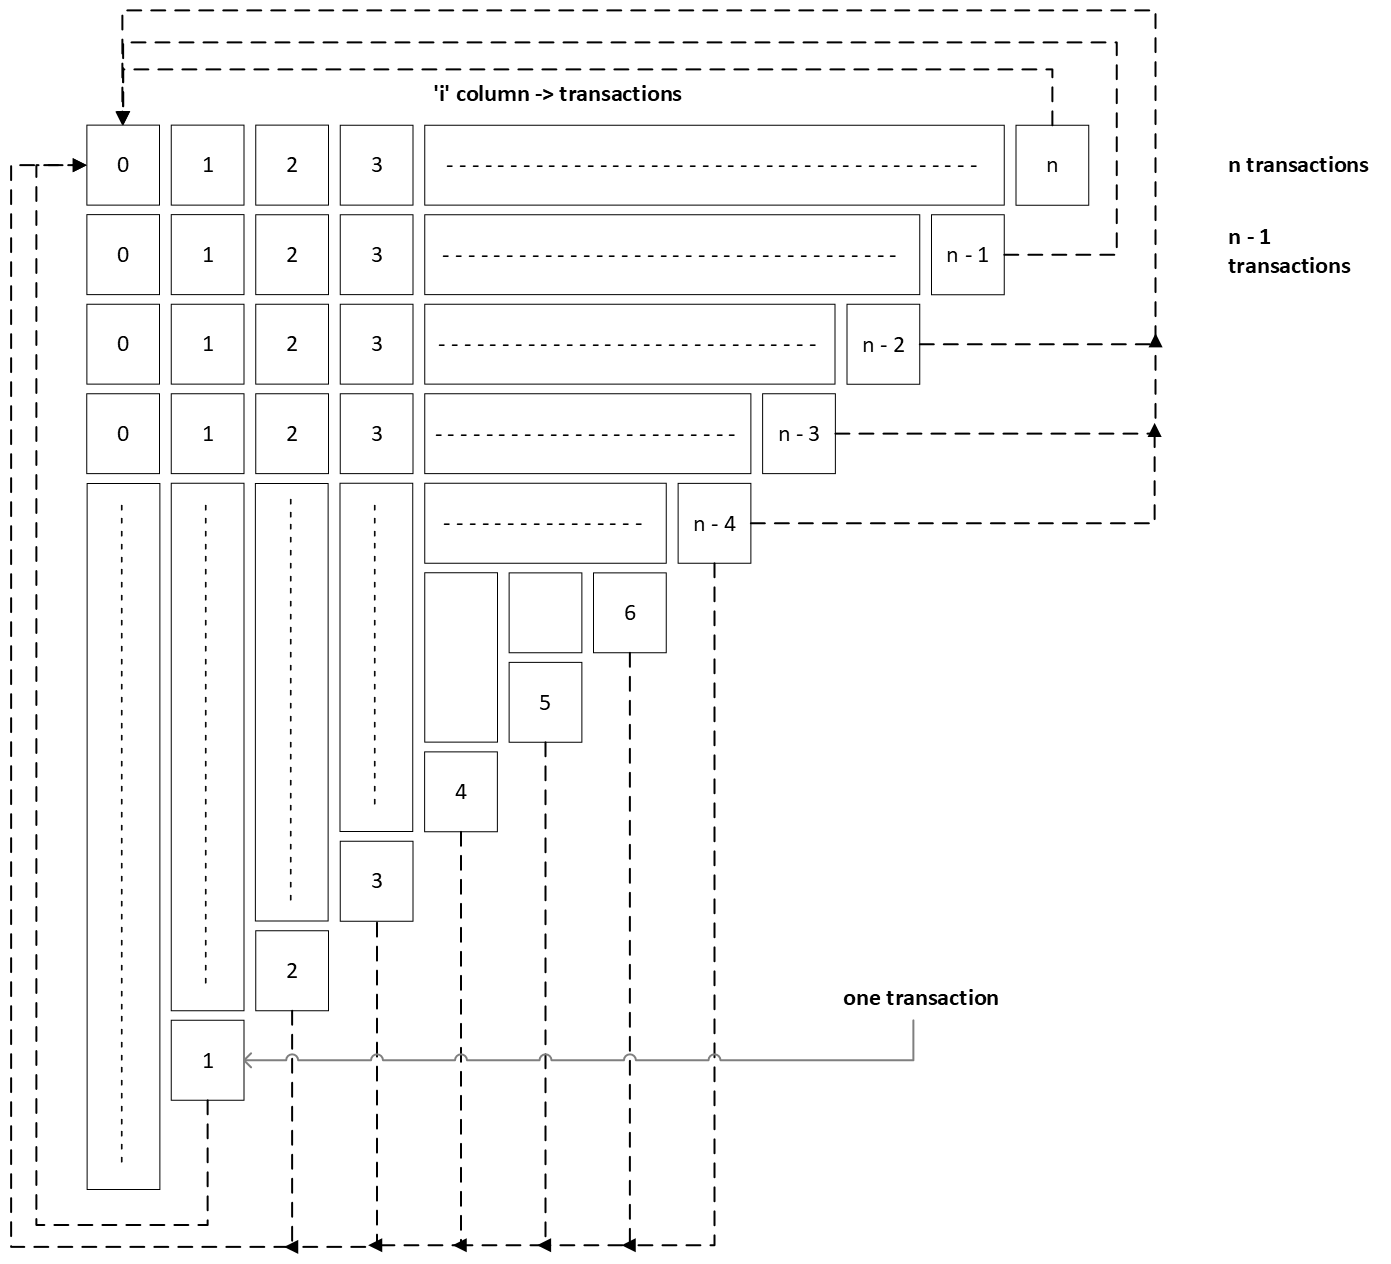
\includegraphics[width=\textwidth]{Figures/FlowDiagram.png}}
    \caption{Flow Diagram of new model.} 
    \label{flow}
\end{figure*}	

Due to the ethereum network switching from the proof-of-work to proof-of-stake 
concept for their consensus algorithm, as discussed in Sec. ~\ref{related}, we have decided to update
the base model in Seol\cite{2020_ACM_Seol} to reflect this new regime. This 
new proof-of-stake methodology essentially flips the previous base model on its 
head, where the time between blocks being pushed out to validators is set at twelve 
seconds, and because of this, the block size (in terms of gas) can then fluctuate based 
on the number of transactions that have arrived in the latest block window of time. 

The subsequently updated variables and assumptions are given below. 

$P_{0,0}$: The state at which no time has passed in the block window of time. 

$P_{t,0}$: The state at all of the time has passed in the block window of time, and
the block is ready to be sent to the validator community, with no slow transactions. 

$P_{t-j,j}$: The state at all of the time has passed in the block window of time, and
the block is ready to be sent to the validator community, with $j$ slow transactions. 

$P_{i,0}$: The state at which $i$ fast transactions have arrived in the 
block window of time with 0 slow transactions. 

$P_{i,j}$: The state at which $i$ fast transactions have arrived in the 
block window of time with $j$ slow transactions. 

$\tau$: The minimum time increment that can pass between the 
fast transaction arrivals. 

$T$: The total time that will pass between each block creation and is initially static.

$t$: The total number of fast transactions that can be seen in one block window of time.
This is calculated as $\frac{T}{\tau}$, therefore if $T$ is fixed at twelve seconds and
$\tau=\frac{1}{32}$ then $t=\frac{12}{\frac{1}{32}}=384$. 

$\Omega$: The rate for the entire block to be posted and purged. This is assumed
to balance the new form of equations as $\mu$ did in the original base model.

$n$: The number of transactions in the block. This is now dependent on $j$ which is
the number of slow transactions that has been seen in the current block window. Here, 
$n=t - j$ or the total possible fast transactions, minus the slow transactions seen in the
block window of time

\subsubsection{$P_{0,0}$} $\\$

\begin{figure}[htbp]
    \centerline{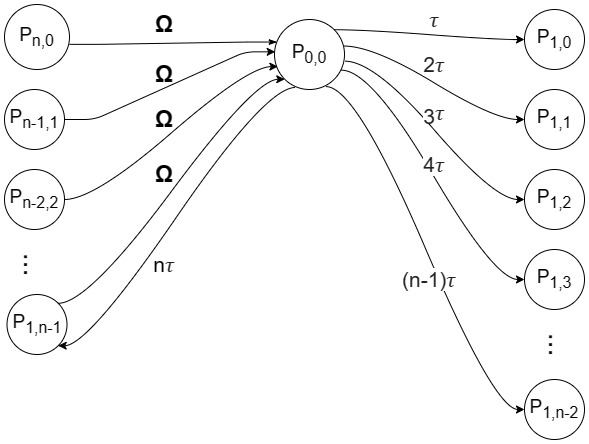
\includegraphics[width=\linewidth]{Figures/StateTransition2.jpg}}
    \caption{State Transition Diagram of $P_{0,0}$} 
    \label{trans1}
\end{figure}	

Incoming from $P_{t,0}$, $P_{t-1,1}$, $P_{t-2,2}$, ... , $P_{2,t-2}$, $P_{1,t-1}$

Outgoing to $P_{1,0}$, $P_{1,1}$, $P_{1,2}$, ... , $P_{1,t-2}$, $P_{1,t-1}$

\begin{multline}
\Omega(P_{t,0} + P_{t-1,1} + P_{t-2,2} + ... + P_{2,t-2} + P_{1,t-1})\\
= \tau(1 + 2 + 3 + ... + t-1 + t)P_{0,0}\label{nm_1}
\end{multline}

Here we have the summation from $1$ to $t$ which can be rewritten as 
$\frac{t(t+1)}{2}$ and the other summation is all of the possible ending states
before we return to $P_{0,0}$. This can then be rewritten in Eq. ~\ref{nm_2}.

\begin{equation}
\Omega\sum_{j=0}^{t-1}{P_{t-j,j}} = \tau\frac{t(t+1)}{2}P_{0,0}\label{nm_2}
\end{equation}

As can be seen here, our added parameter $j$ for the slow transactions has
the effect of splitting the final state, $P_t$ from the base model in 
Seol\cite{2020_ACM_Seol} into various states from $0$ slow transactions up
to $t-1$ slow transactions.

It is with this addition, along chopping a fixed amount of time to minimum time
increments, $\tau$, that we can approximate the proof of stake workflow in 
blockchain networks, like Ethereum. 

\subsubsection{$P_{1,j}$} $\\$

Incoming from $P_{0,0}$ only (with time $(j+1)\tau$)

Outgoing to $P_{2,j}$, $P_{2,j+1}$, $P_{2,j+2}$, ... , $P_{2,t-3}$, $P_{2,t-2}$

\begin{multline}
\bcancel{\tau}(j+1)P_{0,0} = \\
\bcancel{\tau}(1 + 2 + 3 + ... + (t-j-2) + (t-j-1))P_{1,j}\label{nm_3}
\end{multline}

\begin{equation}
P_{0,0} = \frac{(t-j-1)(t-j)}{2(j+1)}P_{1,j}\label{nm_4}
\end{equation}

\subsubsection{Combining Eq. \ref{nm_2} and Eq. \ref{nm_4}}

\begin{multline}
\frac{\cancel{2}\Omega}{\tau (t(t+1))}(P_{t,0} + P_{t-1,1} + P_{t-2,2} + ... \\
+ P_{2,t-2} + P_{1,t-1}) = \frac{(t-j-1)(t-j)}{\cancel{2}(j+1)}P_{1,j}\label{nm_5}
\end{multline}

\begin{multline}
P_{1,j} = \frac{(j+1)\Omega}{\tau(t(t+1))((t-j-1)(t-j))}\\
(P_{t,0} + P_{t-1,1} + ... + P_{1,t-1})\label{nm_6}
\end{multline}

******STOPPING HERE - A LOT OF THESE EQUATIONS MIGHT BE REPLACED TOMORROW - GOING TO BED*******
\subsubsection{$P_{n-j,j}$} $\\$

\begin{figure}[htbp]
    \centerline{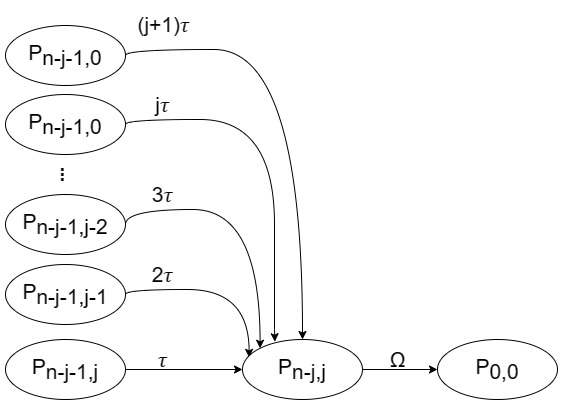
\includegraphics[width=\linewidth]{Figures/StateTransition3.jpg}}
    \caption{State Transition Diagram of $P_{n-j,j}$} 
    \label{trans2}
\end{figure}	

Incoming from $P_{n-j-1,j}$,$P_{n-j-1,j-1}$,...,$P_{n-j-1,1}$,$P_{n-j-1,0}$

Outgoing to $P_{0,0}$

\begin{multline}
\tau(P_{n-j-1,j} + 2P_{n-j-1,j-1} + 3P_{n-j-1,j-2} + ... \\
+ jP_{n-j-1,1} + (j+1)P_{n-j-1,0} = \Omega P_{n-j, j}\label{nm_7}
\end{multline}

\begin{multline}
P_{n-j, j} = \frac{\tau}{\Omega}(P_{n-j-1,j} + 2P_{n-j-1,j-1} + ... \\
+ (j+1)P_{n-j-1,0} \label{nm_8}
\end{multline}

\subsubsection{$P_{i,j}$} $\\$

\begin{figure}[htbp]
    \centerline{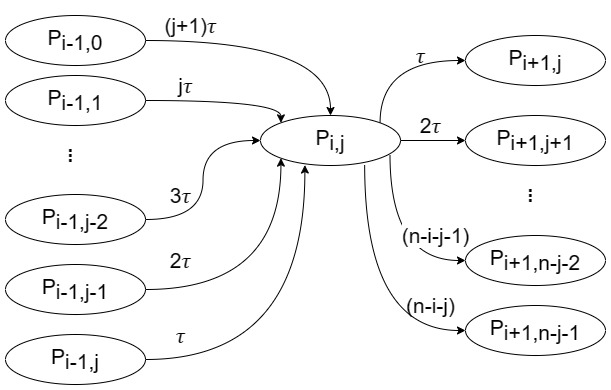
\includegraphics[width=\linewidth]{Figures/StateTransition4.jpg}}
    \caption{State Transition Diagram of $P_{i,j}$} 
    \label{trans3}
\end{figure}

Incoming from $P_{i-1,j}$, $P_{i-1,j-1}$, ... , $P_{i-1,0}$

Outgoing to $P_{i+1,j}$, $P_{i+1,j+1}$, $P_{i+1,j+2}$, ... , $P_{i+1,n-i-1}$

\begin{multline}
\bcancel{\tau}(P_{i-1,j} + 2P_{i-1,j-1} + 3P_{i-1,j-2} + ... + jP_{i-1,1} + \\
(j+1)P_{i-1,0}) = \bcancel{\tau}(1 + 2 + 3 + ... + (n-i-j-1) + \\
(n-i-j)) P_{i,j}\label{nm_9}
\end{multline}

\begin{multline}
P_{i,j} = \frac{2}{(n-i-j)(n-i-j+1)}(P_{i-1,j} + 2P_{i-1,j-1} +  \\
... + (j+1)P_{i-1,0})\label{nm_10}
\end{multline}	

\subsubsection{Constraint: Markovian Queueing Assumption}

\begin{equation}
P_{0,0} + \sum_{i=1}^{n}{\sum_{j=0}^{n-i}{P_{i,j}}} = 1.0\label{nm_11}
\end{equation}

\subsubsection{Remarks} $\\$

$\bullet$ Each $P_{i,j}$ depends on the previous $(i-1)$ column and its 
preceding $(0 ... j)$ rows. This $P_{i,j}$ in turn, affects $P_{i+1,j}$ through
$P_{i+1,n-i-1}$.

$\bullet$ The $i=0$ column has only $P_{0,0}$ (no arrivals and no time 
elapsed.

\subsection{Optimization}\label{optimization}

The main point left to discuss is the optimization problem to set n to an optimum level given what 
the new expectation is for the coming $\lambda$. The new expectation for the coming $\lambda$ will 
be the average of all $\lambda$ that we have seen up until that point, which is an unbiased estimator 
of the random variable $\lambda$ since our model will not have any prior knowledge of the range of 
values to be passed in. 
	
The derivatives of the $\gamma$ and W$_Q$ are difficult to calculate for these purposes, so to approximate 
the derivatives we will use the first differences. This calculation is given by:

\begin{equation}
\Delta \gamma = \gamma[2:n] - \gamma[1:n-1]\label{deltagamma_eq}
\end{equation}

\begin{equation}
\Delta W_Q  = W_Q [2:n] - W_Q [1:n-1]\label{deltawq_eq}
\end{equation}

Since the functions are evaluated at small, discrete, and uniformly spaced time steps the approximation 
should be accurate for our purposes. 

\begin{equation}
optN=argmin f(n):=\{ -nlg(n)\cdot\frac{\Delta \gamma}{\Delta W_Q}\}\label{optn_eq}
\end{equation}

\subsection{Closed Form Optimization}\label{closed_opt}

In this semester, we can start by removing the iterative, numerical process described above with 
a closed form solution to get the optimal n. The first thing then is that we have to look at the metric.
In the iterative process we had the ratio of throughput over waiting time multiplied by a plug of $n lg(n)$. 

Let's then look at the equations of throughput and waiting time to see how the ratio looks when reducing it 
down. W$_Q$ is given in eq. \ref{WQ_eq} as simply L$_Q$ divided by $\lambda$, so lets write that out and 
show that $\lambda$ cancels out in that equation.

\begin{equation}
W_Q=\frac{n\ast\frac{\lambda}{\mu}\frac{n(n+1)}{2}P_0}{\lambda}=n\ast\frac{\cancel{\lambda}}{\mu}\frac{n(n+1)}{2}P_0\ast\frac{1}{\cancel{\lambda}}\label{WQ_reduced}
\end{equation}

Eq. \ref{gamma_eq} gives the equation for $\gamma$, so if we look at the equation for the ratio of throughput over waiting time we get eq. \ref{ratio_eq}. 

\begin{equation}
\frac{\gamma}{W_Q}=\frac{\lambda\cancel{\frac{n(n+1)}{2}}\cancel{P_0}}{\frac{n}{\mu}\cancel{\frac{n(n+1)}{2}}\cancel{P_0}}=\frac{\lambda}{\frac{n}{\mu}}=\frac{\mu}{n}\ast\lambda\label{ratio_eq}
\end{equation}

Now, this ratio when reduced shows that throughput over waiting time is a montonically increasing function, 
with $\mu$ being fixed this means that $n$ is directly dependent on $\lambda$. This would not lead to an optimal 
level of $n$, but rather as $\lambda$ became smaller (or quicker), $n$ would should become smaller. In practice, 
batching was necessary to process transactions more efficiently, so there should be some penalty for having blocks 
that are too small. The particular network or application would probably have a direct impact on this number, but
for our case in an arbitrary blockchain, let's set this to $\frac{1}{3n^3}$. In this way, when $n$ gets very small, 
the penalty gets larger. A maximum can also be determined based on network processing speeds as a cap to 
$n$. So, now we have eq. \ref{metric_eq} which we can denote $M$ for metric.

\begin{equation}
M=\frac{\gamma}{W_Q}-penalty=\frac{\mu\lambda}{n}-\frac{1}{3n^3}\label{metric_eq}
\end{equation}

To find the maximum/minimum of this equation we need to take the first derivative with respect to $n$ 
and set it equal to zero. 

\begin{equation}
\frac{\delta M}{\delta n}=-\frac{\mu\lambda}{n^2}+\frac{1}{n^4}=0\label{metric_deriv}
\end{equation}

Then solving for $n$ we have eqs. \ref{cf_opt_n_1}, \ref{cf_opt_n_2}, \ref{cf_opt_n_3}.

\begin{equation}
-\frac{\mu\lambda}{n^2}=-\frac{1}{n^4}\label{cf_opt_n_1}
\end{equation}

\begin{equation}
\frac{n^4}{n^2}=\frac{1}{\mu\lambda}\label{cf_opt_n_2}
\end{equation}

\begin{equation}
n=\frac{1}{\sqrt{\mu\lambda}}\label{cf_opt_n_3}
\end{equation}

We now have the closed form solution that the optimal block size ($n$) is inversely related to
the square root of the cost of creating a block ($\mu$) times the speed with which the transactions 
are coming into the network($\lambda$). 

Using this same equation, $\lambda$ can also be projected based on the cyclical nature of how transaction
speeds progress throughout the day and the optimal $n$ can be calculated before each block is created to 
predetermine the next block size to be created. 

\section{Results}

TODO: Redo this later

\section{Conclusion}

TODO: Redo this later

\bibliographystyle{IEEEtrans}
\bibliography{Crosby}

\end{document}
